\documentclass[a4paper,titlepage]{article}
\usepackage[utf8]{inputenc}   	% pro unicode UTF-8
\usepackage[czech]{babel} 		%jazyk dokumentu
\usepackage{listings}
\usepackage{color}
\usepackage[T1]{fontenc}
\usepackage{hyperref}
\usepackage{listingsutf8}
\usepackage{graphicx}
\usepackage{subcaption}
\usepackage[font=small,labelfont=bf]{caption}
\usepackage{lipsum}

\graphicspath{ {/} }

\definecolor{lightgray}{rgb}{.9,.9,.9}
\definecolor{darkgray}{rgb}{.4,.4,.4}
\definecolor{purple}{rgb}{0.65, 0.12, 0.82}
\lstdefinelanguage{javascript}{
  keywords={typeof, new, true, false, catch, function, return, null, catch, switch, var, if, in, while, do, else, case, break},
  keywordstyle=\color{blue}\bfseries,
  ndkeywords={class, export, boolean, throw, implements, import, this},
  ndkeywordstyle=\color{darkgray}\bfseries,
  identifierstyle=\color{black},
  sensitive=false,
  comment=[l]{//},
  morecomment=[s]{/*}{*/},
  commentstyle=\color{purple}\ttfamily,
  stringstyle=\color{red}\ttfamily,
  morestring=[b]',
  morestring=[b]"
}
\lstset{
   language=javascript,
   backgroundcolor=\color{lightgray},
   extendedchars=true,
   basicstyle=\footnotesize\ttfamily,
   showstringspaces=false,
   showspaces=false,
   numbers=left,
   numberstyle=\footnotesize,
   numbersep=9pt,
   tabsize=2,
   breaklines=true,
   showtabs=false,
   captionpos=b
}

\title{
	Dokumentace\\
	\textbf{Snake ve 3D}
}
\author{
	\textbf{David Nápravník}\\
	Matematicko-fyzikální fakulta\\
	Univerzita Karlova\\
	Programování a softwarové systémy
}
\date{2018}

%%%%%%%%%%%%%%%%%%%%%%%%%%%%%%%%%%%%%%%%%%%%%%%%%%%%%%%%%%%%%

\begin{document}
	\maketitle
	\tableofcontents
	\newpage
	
	\section{Úvodní slovo}
	\subsection{Úvod do problematiky}
		Projekt Snake ve 3D je jednoduchá hra, jež je vylepšenou verzí klasické hry Snake z 90.let.\cite{Snake-wikipedie}\\
		Hlavním vylepšením je přenesení hry do prostoru o třech dimenzích, jež nejsou ohraničené, tudíž se
		jedná o nekonečný svět v němž se had (naše postavička) může pohybovat bez omezení.\\
		Dalším vylepšením je přidáním dalších hadů do herního světa jež řídí počítač.
	\subsection{Uživatelská Příručka}
		Po načtení stránky a všech dalších komponent hra začíná.\\
		Vaším úkolem je sbírat jídlo, jež je reprezentováno krychlí, ležící na viditelných osách.\\
		Pro pohyb hada jsou vyhrazeny klávesy WASDQE.		
		\begin{table}[ht]
			\begin{tabular}{ll}
				W	&	náklon nahoru\\
				A 	& 	otočení doleva\\
				S 	&	náklon dolu\\
				D 	& 	otočení doprava\\
				Q 	& 	rotace doleva\\
				E 	& 	rotace doprava
			\end{tabular}
		\end{table}
		\\
		Pro přidání hada do hry slouží klávesa "+" a pro odebrání klávesa "-"
		Při nárazu hlavou do jakéhokoliv (i svého) ocasu se vám odebere jeden život ze tří.
		Při nulovém stavu života hra začíná od začátku.
		Hra nemá žádný pevně daný konec, tudíž ji můžete hrát až nekonečně dlouho.\\
		
		\includegraphics[width=11cm]{screen.jpg}
		\\		
		V pravo nahoře je skóre, neboli délka hada.\\
		Barva určuje o kterého hada se jedná.\\
		V levém horním okraji se na chvíli zobrazí manuál k ovládání a
		po deseti vteřinách zmizí, aby nepřekážel ve výhledu.\\
		Vlevo dole jsou pak životy vašeho hada, popřípadě hláška, že životy nemáte.\\
		Uprostřed obrázku je vidět jídlo (malá zeleno bílá věc) jež leží na 3 pomocných čárách
		(na každé ose jedna)\\
		Dále zde vydíme našeho hada (modrý) a tři hady řízené počítačem (žlutí).
		Neprúhledná krychle značí hlavu, naopak poloprůhledná značí ocas.
		
				
		
	\subsection{Programovací jazyk}
	\subsubsection{Javascript\cite{JavaScript-wikipedie}}
		Při výběru jazyka nebylo moc možností. Jelikož se jedná o webovou
		aplikaci je téměř nutností použít jazyk javascript pro veškeré výpočty.
		API pro renderování používá jazyk GLSL pro práci s shadery ve webGL.\\
		Javascript je dynamicky typovaný jazyk postavený na objektech.\\
		Pro tento program používám verzi ECMAScript 6.
		Tudíž je kompatibilní s většinou nových prohlížečů.
		Podporovány jsou Crome, Firefox, Edge.
		K nepodporovaným patří Internet Explorer, jež nemá dostatečně dobře implementováno webGL\cite{webGL}.
	\subsection{BABYLONJS}	
		BABYLONJS je webové API napsané v javascriptu (nebo v typeScriptu) a
		jazyku GLSL pro práci se shadery na grafické kartě pomocí webgl.\\
		Knihovna je zdarma a v mnoha podobách na stránkách www.babylonjs.com\cite{BabylonJS}.
		Knihovna se dá importovat buď online a
		tak se vždy stahuje nejaktuálnější stabilní verze, nebo
		se dá stáhnout a umístit na vlastní webové úložiště.
		Ke stažení je mnoho variant s podporou Fyziky, nebo defaultními texturami a Kolizemi.
		Knihovna se dá stáhnout buď "ukecaná" nebo minimalizovaná.
		Pro tento projekt je použita "Offline" minimalizovaná verze bez jakýchkoliv nadstaveb, jednoduše čisté BABYLONJS.
	\subsubsection{Implementace}
		Knihovna je zcela zapouzdřená a každé její volání má předpodu \textit{BABYLON}.\\
		Pro počáteční nastavení je nejdůležitější nastavit scénu a kameru.\\
		Scéna je objekt uchovávající veškeré další objekty potřebné pro vykreslování, včetně kamery a enginu.\\
		\\
		\textbf{Kamera}\\
			Podle typu kamery se použije daný způsob vykreslování a pohybu popř. rotace. Knihovna nabízí tyto kamery:
			\begin{itemize}
			\item Universal Camera
			\item Arc Rotate Camera
			\item FollowCamera
			\item AnaglyphCameras
			\item Device Orientation Camera
			\item VR Device Orientation Cameras
			\item Free Camera
			\end{itemize}
			Nejpoužívanějším typem je \textit{Univerzal Camera}, ta ovšem nepodporuje otáčení po ose \textit{z}.
			Arc Rotate Camera je spíše pro statické modely, které se nepohybují. FollowCamera by pro tento projekt byla zcela
			nejvýhodnější možnost, protože bych se nemusel pitvat s manuálním sledováním hlavy hada, ale
			i tak tato možnost plně nezahrnuje funkce jenž jsem pro projekt požadoval.
			AnaglyphCameras a VR Device Orientation Cameras slouží pro 3D obraz, což bez speciálních brýlí stejně není možné.
			Jak název napovídá Device Orientation Camera otáčí kamerou tak jak je nakloněno hostující zažízení
			(např. mobilní telefon s G-senzorem).\\
			Ačkoliv Free Camera nedělá téměř nic automaticky, tak se dá doprogramovat tak aby dělala zcela vše potřebné
			a tudíž se stala jedinou použitelnou. Umí rotaci po všech třech osách, polohu a fov (field of view)\cite{field of view}.\\
			\\
		\textbf{Světlo}\\
			Aby při vykreslování nebylo vidět jen černo je potřeba přidat do scény světlo.
			Vykreslovací engine pak spočítá odraz světla od tělesa na pomocné pláno.
			Ačkoliv BABYLON nabízí hromadu možností světel a jejich vlastností, není potřeba nic speciálního,
			takže stačí světlo typu \textit{HemisphericLight}.\\	
			\\
		\textbf{SkyBox}\cite{Skybox}\\
			V každé 3D hře se používá tkz. skybox, jedná se o krychly několika násobně větší než celý herní svět.
			Vnitřní stěny mají texturu nebe (nebo jiného prostředí) a pomocí optické iluze to vypadá jako reálné nebe.
			Tento trik je velmi efektivní a výpočetně nenáročný.\\
			\begin{center}	
				\includegraphics[width=5cm]{space_skybox_by_orindoomhammer.jpg}
				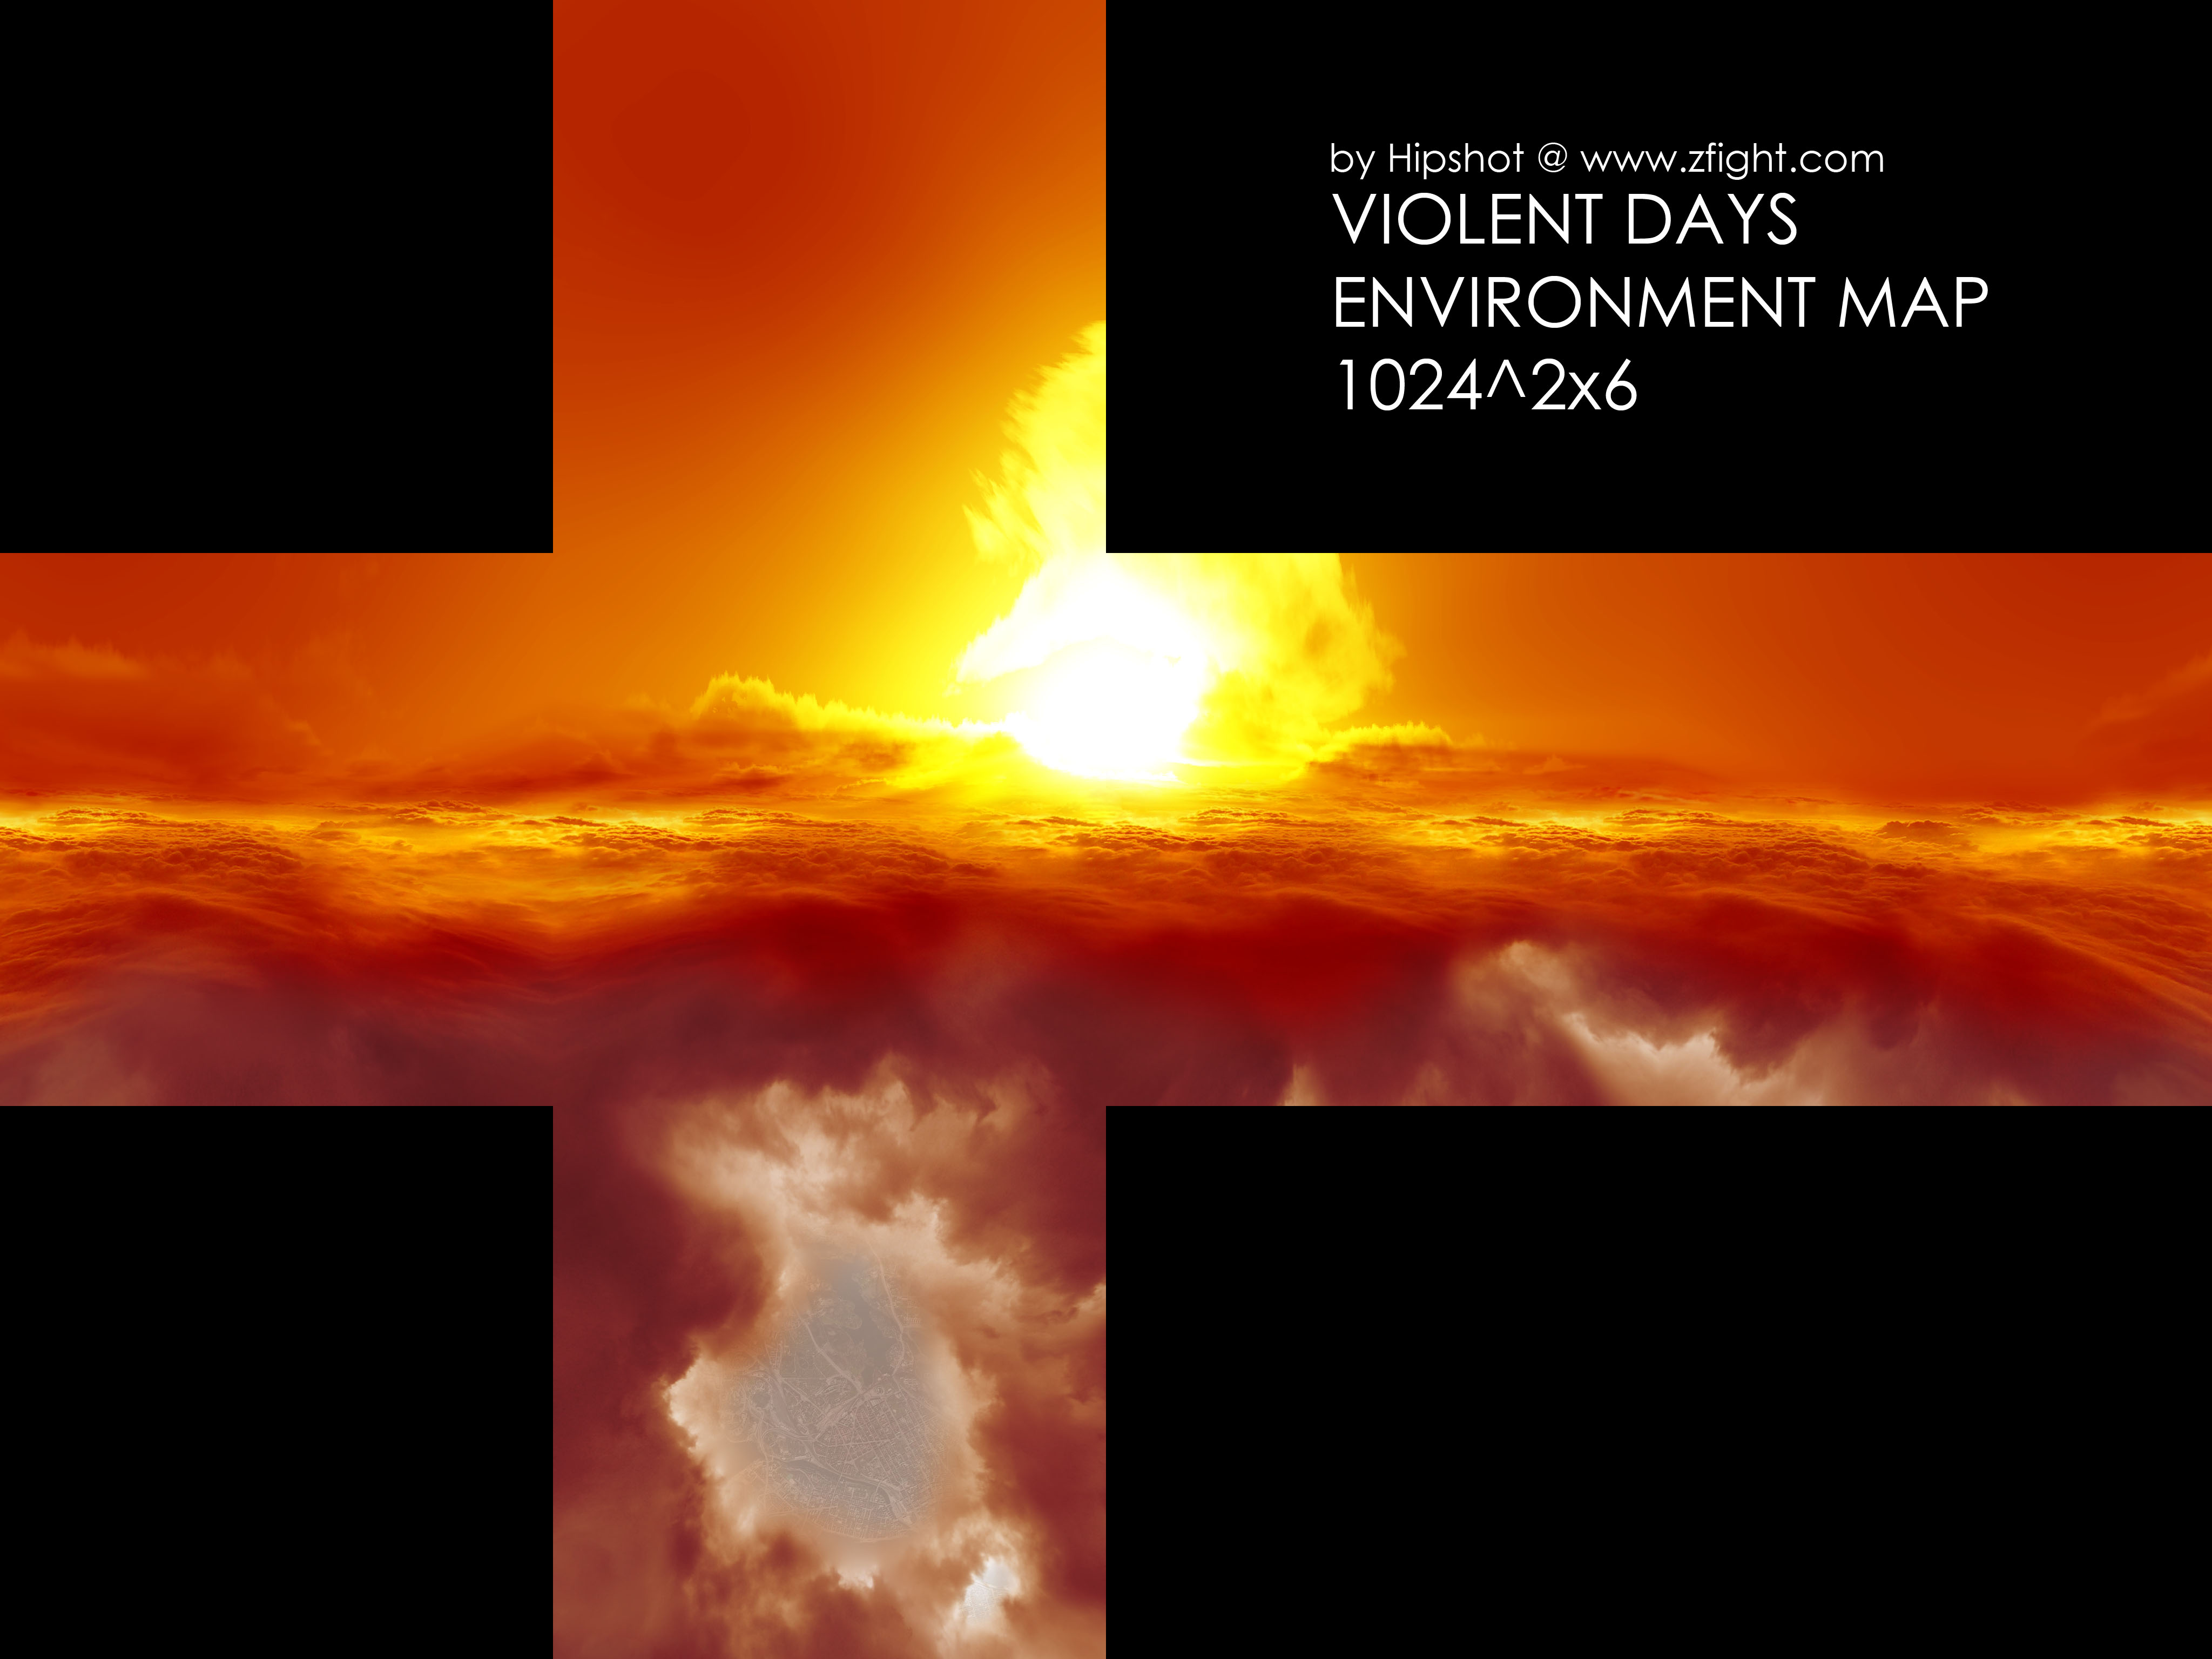
\includegraphics[width=5cm]{violentdays_large.jpg}	\\
				příklad textur pro skybox\\
				
				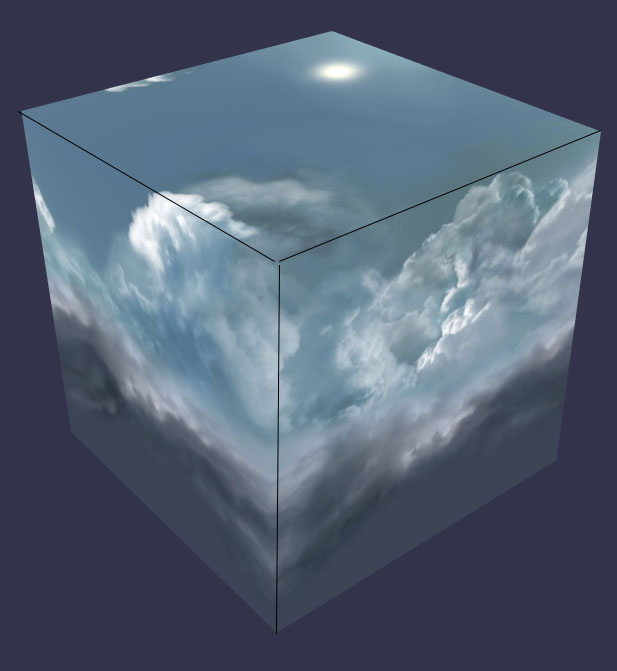
\includegraphics[width=5cm]{skybox.jpg}\\
				aplikovaná textura v paxi. (hodně oddáleně)
			\end{center}		
				
			
		\textbf{Material}\\
			Jakémukoliv tělesu se dá přiřadit materiál, jež poté určuje vlastnosti tělesa a to jak vypadá.
			Hlavními vlastnostmi materiálu jsou:
			\begin{itemize}
				\item Barva
				\item Textura
				\item Průhlednost
				\item Odrazivost světla
			\end{itemize}	
	\section{Datový návrh}
	\subsection{Konstruktory}
		Vetšina objektů má vlastní konstruktory aby se dali snadno vytvářet další jejich kopie a
		aby jednotlivé komponenty byly zapouzdřené. Zde je výčet těch nejdůležitějších.
	\subsubsection{Food}
		Na vstup bere parametry x,y,z jež reprezentují celočíselné souřadnice umístění jídla v 3D prostoru.
		Další parametr je počet bodů jež had získá po snězení tohoto jídla.
		Parametr obj je objekt krychle z BABYLONJS.
		Parametr lines jsou 3 vodící čáry jež pomáhají nalézt jídlo ve 3D
		a mají délku 50 jednotek na každou stranu.
		Konstruktor dále vytváří design jež reprezentuje barvu potravy.
		Design je objekt typu Material z BABYLONJS
	\subsubsection{Part}
		Jednoduchý konstruktor pro vytváření čĺánků ocasu hada.
		Bere x,y,z, design a velikost, jež je součástí designu a vytváří objekt krychle pomocí BABYLONJS
	\subsubsection{Design}
		Slouží pro propojení herního materiálu a materiálu pro vykreslování pomocí BABYLONJS.
		Dle typu se vytvoří materiál pro hada nebo jídlo.
		Barva se předává pomocí objektu typu: \{r:-barva-,g:-barva-,b:-barva-\}.
	\subsubsection{Snake}
		Snake je Objekt z něhož dědí SnakePlayer a SnakeComputer.\\
		Obsahuje informace jež jsou pro oba typy hadů společná jako jsou:\\		
		\begin{itemize}
			\item Barva
			\item Design jež je popsán výše.
			\item Pozici hlavy na mapě, ve formátu \{x,y,z,objekt newSnakePiece\}
				newSnakePiece je objekt z BABYLONJS jež reprezentje krychly, v našem případě hlavu hada
			\item Pole dílků hada
			\item Boolean hodnota zda had právě jedl (důležité kvůli pozdějšímu přidávání dílků hada)		
		\end{itemize}
		Dále společnou metodu:\\
		\begin{itemize}
			\item Eat jež prodlouží hada a poté vymaže staré jídlo a vytvoří nové na nových souřadnicích\\				
		\end{itemize}
		Nakonec se vytvoří základních 10 dílků hada.
	\subsubsection{SnakePlayer}
		Dědí z objektu Snake.\\
		Oproti počítači má hráč 3 životy namísto jednoho.\\
		Informace o směru a rotaci, aby se hráč lépe zorientoval.\\
		Metodu move, jež má na starost:\\
		\begin{tabbing}
			kontrola zda jsme nenašli jídlo\\
			srážku s čímkoliv jinym pomocí funkce srazkaSOcasem()\\
			zrotování dle hráče\\
			přesun hlavy a těla na další políčka\\
			kontrola zda se hráčův had nedostal moc daleko od jídla 
		\end{tabbing}	
		Metody rotate a turn slouží k otáčení a transformaci hada, jež jsou vysvětleny níže.		
	\subsubsection{SnakeComputer}		
		Dědí z objektu Snake.\\
		Oproti hráči zde neřešíme jak je hadí hlava otočena, proto zde stačí ji přesouvat jako všestraně souměrnou krychly.\\
		Metoda removeSelf() efektivně z-eliminuje sama sebe a vymaže aktuálního hada z aktivních hadů v poli snakes[]
	\section{Herní mechanismus}
		Celá hra běží většinou na 60 fps, což je omezeno interpretem javaScriptu,
		jež rychlejší vykreslování nepovoluje.
		Čas ve hře je ukládán pomocí Ticků hry a ne pomocí reálného času,
		tudíž pokus klesne rychlost vykreslování,
		kvůli nízkému výkonu stroje (sníží se FPS), pak se zpomalí i pohyb hada po mapě.
		Což je obrana proti nechtěnémupřeskočení herních mechanismů.
		Proměnná \textit{hardwareClock} ukládá počet Ticků od začátku hry.
		Tato proměnná se dále modulí rychlostí hry uložené v \textit{gameSettings.speed}
		a získáme aktuální Tick mezi jedním pohybem hadam a uložíme jej do proměnné \textit{betTick}.
		\textit{betTick} nám dále poslouží k rozložení výkonu do více Ticků, takže se eliminuje efekt,
		kdy jeden Tick se bude počítat několika-násobně déle, než Ticky ostatní.\\
		\\
		V každém Ticku se zavolají všichni hadi, aby provedli pohyb. Hadi se volají od čísla 0, což je hráč, až
		po celkový počet hadů, jež je ve hře.\\
		Na konci se upraví pozice a rotace kamery tak, aby hráč (Uživatel) měl nejlepší rozhled o všem co se děje.
		Takže kamera "létá" kousek za hlavou hada a je natočená na pozici kam had směřuje. 
	\subsection{Uživatel}
		Hráčův had je plně kontrolován uživatelem a jeho pohyb závisí na stisknutých klávesách.
		Stisky kláves se ukládají do fronty FIFO a při každém Ticku jež je pro hada předělový
		(Když se had pohne z jednoho políčka na jiné, většinou betTick 0)
		se jedna klávesa zprauje a ostatní čekají na další zavolání.
	\subsubsection{Rotace a orientace}
		Pohyb hada je řízen pomocí rotace kolem krychle a směrem.
		Náš had má hlavu krychle, ta slouží jako hlavní orientační objekt pro celý pohyb hada.\\
		Každá rotace hlavy se dá popsat jako otočení krychle, neboli otočení jedné stěny směrem nahoru.
		Krychle má 6 stran jež i zároveň reprezentují 3 osy v prostoru (x,y,z).
		Dalším orientačním prvkem je směr kam se z dané strany koukáme, tyto strany jsou 4.
		Krychle má na opačných stranách součet čísel 7, což znamená, že pokud jsme na straně x pak
		spodní strana má číslo 7-x.
		\begin{lstlisting}[language=javascript]
			case 'W': 
				this.direction.d=staraStrana;
				break;
			case 'S': 
				this.direction.d=7 - staraStrana;
				break;
		\end{lstlisting}		
		Z jedné stěny tudíž lze vidět všechny strany jež nejsou rovny x nebo 7-x.
		Tyto stěny jsou vypočítany pomocí matice ve funkci \textit{prepoctiHranu()}
		\begin{lstlisting}[language=javascript]
			function prepoctiHranu(dir,rot){
				var krychle=[
					[0,3,5,2,4,0],
					[4,0,1,6,0,3],
					[2,6,0,0,1,5],
					[5,1,0,0,6,2],
					[3,0,6,1,0,4],
					[0,4,2,5,3,0]
				];
				return krychle[dir-1][rot-1];
			}
		\end{lstlisting}
		Dle stěny krychle a směru další hrany můžeme určit směr kam se had (jeho hlava) pohybuje.\\
		 
	\subsection{Počítač}
		Do herního světa lze přidat neomezené množství dalších hadů, jež jsou řízeny počítačem.
		Algoritmus pro řízení je optimalizován pouze pro vítězství bez ohledu na uživatele a 
		nedává mu žádné výhody. Uživatel tedy hraje proti čisté síle stroje. A výkon není omezen ani časem výpočtu.
	\subsection{Herní nastavení}
		Nejhlavnější možnosti hry jsou uloženy v objektu \textit{gameSettings}, ty se dají upravit dle potřeby.
		Nejdůležitější je však rychlost pohybu hada a rychlost otáčení kamery.
		Základní rychlost hry je 10, což vyjadřuje počet Ticků potřebných k jednomu kroku hry
		(kdy se had posune přesně o jedno políčko).
		Pokud hra běží na 60 FPS (stroj má dostatečný výkon), pak to odpovídá posun hada o 6 (60/10) políček za vteřinu.
		Toto tempo je pro hru nejvhodnější, ale můj názor je relativní, jelikož už jsem si na to zvykl,
		avšak pro uživatele, který tuto hru vidí poprvé je hra velmi rychlá hůře ovladatelná.
	\section{Co by se dalo vylepšit}
		Jelikož se jedná o webovou aplikaci, tak se nabízí možnost multiplayeru,
		neboli připojení více Uživatelů do jedné instanci hry. Jednalo by se o volání AJAXem na server,
		a v databázi by se ukládala poloha všech hadů. Jelikož je tick hry celkem dlouhý (časově), tak by latence
		nebyla takový problém jako u hry žánru FPS.\\
		\\
		Jak mi bylo řečeno jedním z testerů, pro hru je důležitá atmosféra, hudba a děj.
		Ačkoliv děj mi nepřijde zrovna vhodný tak přidáním hudby a zvukových efektů, by hra dostala nový rozměr.\\
		\\
		Dala by se přidat funkce která hada dočasně zrychlí a poskytne mu pak výhodu oproti neomylnému počítači.
		S tím také souvisí práce s fov, jež dokáže onu rychlost uživateli znázornit.\\
		\\		

		
	\begin{thebibliography}{99}
		\bibitem{Snake-wikipedie}
			Snake-wikipedie:\\
			\textit{\href{https://en.wikipedia.org/wiki/Snake_(video_game_genre)}
				{https:\/\/en.wikipedia.org\/wiki\/Snake\_(video\_game\_genre)}}
		
		\bibitem{BabylonJS}
			BabylonJS:\\
			\textit{\href{https://www.babylonjs.com/}
				{www.babylonjs.com}}
			
			
		\bibitem{JavaScript-wikipedie}
			JavaScript-wikipedie:\\
			\textit{\href{https://cs.wikipedia.org/wiki/JavaScript}
				{cs.wikipedia.org/wiki/JavaScript}}
				
		\bibitem{webGL}
			webGL:\\
			\textit{\href{https://cs.wikipedia.org/wiki/WebGL}
				{cs.wikipedia.org/wiki/WebGL}}
				
		\bibitem{field of view}
			field of view:\\
			\textit{\href{https://en.wikipedia.org/wiki/Field_of_view}
				{en.wikipedia.org/wiki/Field\_of\_view}}
				
		\bibitem{Skybox}
			Skybox:\\
			\textit{\href{https://en.wikipedia.org/wiki/Skybox_(video_games)}
				{en.wikipedia.org/wiki/Skybox\_(video\_games)}}
				
	\end{thebibliography}
		
\end{document}
